\documentclass[border=3pt]{standalone}
% Shared preamble for every generated figure.
% Matches the report: newtx (Times), greyscale, square boxes.
\usepackage{newtxtext,newtxmath}
% newtx's typewriter (txtt) draws a slashed zero; use Latin Modern instead.
\renewcommand{\ttdefault}{lmtt}
\usepackage{tikz}
\usetikzlibrary{positioning,arrows.meta,calc,fit,backgrounds,shapes.geometric,
                decorations.pathreplacing,decorations.pathmorphing,matrix,patterns}

\definecolor{figgrey}{gray}{0.88}
\definecolor{figmid}{gray}{0.60}
\definecolor{figdark}{gray}{0.35}

\tikzset{
  fig/.style={font=\small},
  box/.style={draw,thick,minimum height=8mm,minimum width=22mm,align=center,
              inner sep=2pt,font=\small},
  greybox/.style={box,fill=figgrey},
  smallbox/.style={draw,minimum height=6mm,minimum width=16mm,align=center,
                   inner sep=2pt,font=\scriptsize},
  ln/.style={-{Stealth[length=2.2mm,width=1.8mm]},thick},
  lnb/.style={{Stealth[length=2.2mm,width=1.8mm]}-{Stealth[length=2.2mm,width=1.8mm]},thick},
  lbl/.style={font=\scriptsize,inner sep=1.5pt},
  note/.style={font=\scriptsize\itshape,inner sep=1.5pt},
}

\begin{document}
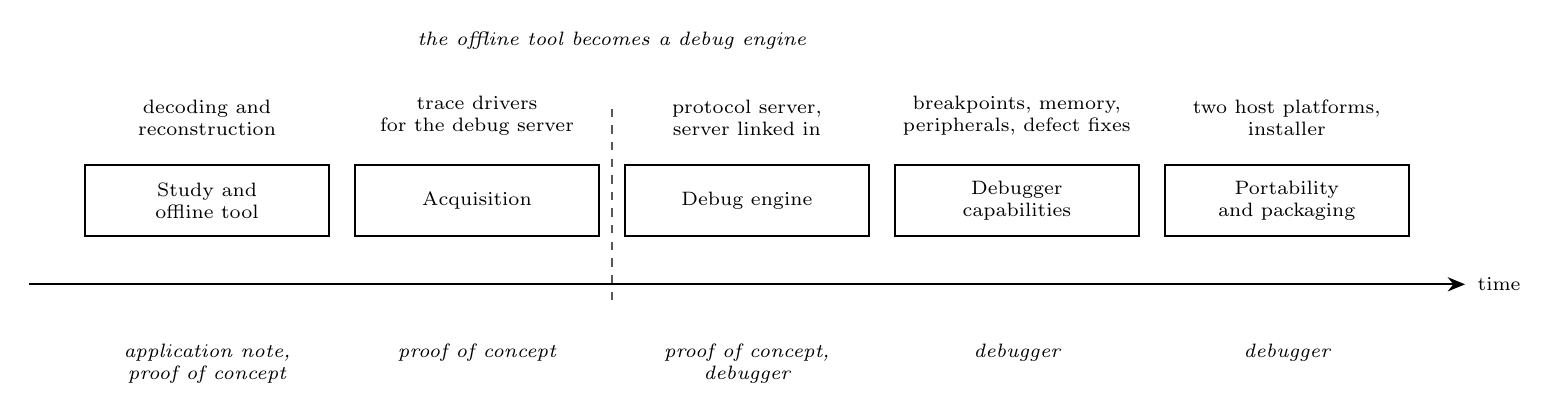
\begin{tikzpicture}[fig,
  ph/.style={draw,thick,minimum height=9mm,minimum width=31mm,align=center,font=\scriptsize},
  res/.style={font=\scriptsize,align=center,inner sep=1.5pt},
  del/.style={font=\scriptsize\itshape,align=center,inner sep=1.5pt}]

\node[ph] (p1) at (0,0)     {Study and\\offline tool};
\node[ph,right=3mm of p1] (p2) {Acquisition};
\node[ph,right=3mm of p2] (p3) {Debug engine};
\node[ph,right=3mm of p3] (p4) {Debugger\\capabilities};
\node[ph,right=3mm of p4] (p5) {Portability\\and packaging};

\draw[ln] ($(p1.south west)-(7mm,6mm)$) -- ($(p5.south east)+(7mm,-6mm)$)
      coordinate[pos=1] (tend);
\node[lbl,anchor=west] at ($(tend)+(1mm,0)$) {time};

\node[res,above=3mm of p1] {decoding and\\reconstruction};
\node[res,above=3mm of p2] {trace drivers\\for the debug server};
\node[res,above=3mm of p3] {protocol server,\\server linked in};
\node[res,above=3mm of p4] {breakpoints, memory,\\peripherals, defect fixes};
\node[res,above=3mm of p5] {two host platforms,\\installer};

\node[del,below=13mm of p1] {application note,\\proof of concept};
\node[del,below=13mm of p2] {proof of concept};
\node[del,below=13mm of p3] {proof of concept,\\debugger};
\node[del,below=13mm of p4] {debugger};
\node[del,below=13mm of p5] {debugger};

\draw[figdark,thick,dashed] ($(p2.north east)!0.5!(p3.north west)+(0,7mm)$)
                         -- ($(p2.south east)!0.5!(p3.south west)+(0,-9mm)$);
\node[note,anchor=south] at ($(p2.north east)!0.5!(p3.north west)+(0,14mm)$)
     {the offline tool becomes a debug engine};

\end{tikzpicture}
\end{document}
